%%%%%%%%%% OPENRISC   %%%%%%%%%%%%%%%%
\chapter{Análisis del microprocesador OpenRISC}
	\section{Introducción}
	El proyecto OpenRISC apunta al desarrollo de arquitecturas RISC de propósito general. OpenRISC 1000, desarrollada por OpenCores, describe una
	familia de procesadores de 32 y 64-bits con procesamiento opcional de punto flotante y vectores.\cite{etiqueta_OR_01}. Su primera implementación
	llamada OpenRISC 1200 (OR1200), escrita en Verilog fue diseñada bajo licencia LGPL con modelos y firmware bajo licencia GPL. 
	
	El OR1200 es un RISC escalar con microarquitectura Harvard, un pipeline de enteros de 5 etapas, soporte de memoria virtual (MMU) y capacidades DSP
	básicas. Las memorias cache por defecto son directas, de 1 vía con 8KB de datos y 1 vía con 8KB de instrucciones respectivamente, cada  una con
	16-bytes de tamaño de línea. Son implementadas inicialmente y constituidas por un TLB de datos de 1 vía y 64 entradas basada en hash en conjunto con
	una TLB de instrucciones de 1 vía y 64 entradas basada en hash. Incluye una unidad de debug de tiempo-real, tick timer, controlador de interrupciones
	programable y soporte para el manejo de energía. La mayoría de sus características pueden ser configuradas por el usuario.
		
	\section{Arquitectura}
	
	La arquitectura OR1000 se basa en la arquitectura del DLX, que es similar a la arquitectura del primer MIPS (MIPS-I). Posee un espacio de direcciones
	lógicas lineal de 32 o 64 bits y espacio de direcciones físicas de implementación opcional. Utiliza un formato de instrucciones simple y de largo
	uniforme en 4 versiones:
	
	\begin{itemize}
	  \item  Set de instrucciones Básico de OpenRISC (ORBIS 32/64) con instucciones de 32 bits alineados en memoria operando con datos de 32 o 64
	  bits.
	  \item Extensión para vectores y DSP (ORVDX64) con instrucciones de 32 bits alineados en memoria operando con datos de 8,16,32 y 64 bits.
	  \item Extensión de punto flotante (ORFPX32/64) con instrucciones de 32 bits alineados en memoria y operandos de 32 y 64 bits.  
	\end{itemize}
	
	Posee dos modos de direccionamiento de memoria: la primera mediante la suma de un operando registro y un inmediato de 16 bits mientras que la segunda
	se realiza sumando un operando registro y un inmediato de 16 bits seguido de una actualización del operando registro con la dirección efectiva
	calculada. La mayor parte de las instrucciones tienen 2 operandos registro (o un registro y una constante). Utiliza retardo de salto (branch delay
	slot) para mantener el pipeline lo mas completo posible. Provee soporte para caches/MMUs de datos e instrucciones separadas (Arquitectura Harvard) y
	para caches/MMUs de datos e instrucciones unificadas (Arquitectura Stanford). Soporta cambios de contexto rápidos en registros, caches y MMUs.
	  
	La arquitectura general consiste en una serie de bloques presentados en la figura ~\ref{fig:ArqOR1200}.
		
	\begin{figure}[h!]
 	\begin{center}
  	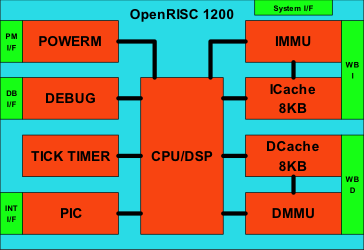
\includegraphics[width=0.5\textwidth,keepaspectratio=true]{./images/OR1200}
  	\caption{Arquitectura del OR1200}
  	\label{fig:ArqOR1200}
 	\end{center}
	\end{figure}

	\subsection{Bloque central CPU/FPU/DSP}

	
	La figura ~\ref{fig:cpufpudsp} muestra el diagrama del bloque básico de CPU/DSP , no se muestras los componentes de la FPU. El OR1200 solo
	implementas secciones de los ISA ORBIS32 y ORFPX32. 

	
	\begin{figure}[!h]
 	\begin{center}
  	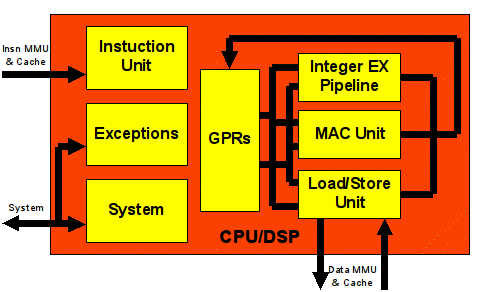
\includegraphics[width=0.5\textwidth,keepaspectratio=true]{./images/cpu_fpu_dsp}
  	\caption{Bloque central del OpenRISC 1200}
  	\label{fig:cpufpudsp}
 	\end{center}
	\end{figure}
	
	\subsection{Cache de datos}
	En la configuración por defecto se tiene una Cache directa de 1 vía con 8KB de extensión. Sin embargo ésta puede ser configurada en alguno de los
	modos listados en la tabla ~\ref{tab:cachedatos} 
	
		\begin{table}[h]
		\centering
		\begin{tabular}{ p{10cm} p{5cm}}
		\rowcolor[gray]{0.8} Modo & Espacio\\
		\hline 
		16B/linea, 256 lines, 1 vía & 4KB\\
		\hline
		16B/linea, 512 lines, 1 vía & 8KB (por defecto)\\
		\hline
		16B/linea, 1024 lines, 1 vía & 16KB\\
		\hline 
		32B/linea, 1024 lines, 1 vía & 32KB\\
		\hline
		\end {tabular}
		\caption{Modos de configuración de la cache de datos del OR1200}
		\label{tab:cachedatos}
		\end {table}
		
	\subsection{Direct-mapped instruction cache}
	
	
	
	\subsection{Data MMU based on hash based DTLB}
	
	
	\subsection{Instruction MMU based on hash based ITLB}
	
	
	\subsection{Power management unit and power management interface}
	
	
	\subsection{Tick timer}
	
	
	\subsection{Debug unit and development interface}
	
	
	\subsection{Interrupt controller and interrupt interface}
	
	
	\subsection{Instruction and Data WISHBONE host interfaces}
	
	
	
	\section{Set de instrucciones}
	
	
	
	\section{Implementación}
		\subsection{ORPSoC}
		\subsection{MinSoc}
	\section{Toolchain}
	\section{Software}
		\subsection{Librerías}
		\subsection{Sistema Operativo}